% !TeX root = protokoll.tex
\PassOptionsToPackage{titlesec}{newparttoc}
\documentclass[ngerman,leqno,x11names]{uol-physics-report}

\partner{Hendrik Philip}{Gorka}{hendrik.philipp.gorka@uni-oldenburg.de}{6478477}
\partner{Jan Eike}{Suchard}{jan.eike.suchard@uni-oldenburg.de}{5945617}
\partner{Terje}{Zirks}{terje.zirks@uni-oldenburg.de}{6417547}
\group{2}
\module{phy215}{Grundpraktikum Physik \rom{2} -- für 2-Fach-Bachelor}
\semester{Sommersemester 2023}
\tutor{Christoph Plaßmeyer}
\supervisor{Marcel Behrens}

\makeatletter
\@addtoreset{section}{part}
\makeatother 

\usepackage{menukeys}
\usepackage{csquotes}
\usepackage{biblatex}
\usepackage{listings}
\usepackage{subcaption}
\usepackage{enumitem}
\usepackage{tcolorbox}
\usepackage{xcolor}
\usepackage{tabularx}
\usepackage{subfiles}

\captionsetup{font=footnotesize, format=hang}

\addbibresource{../global-sources.bib}
\addbibresource{sources.bib}

\graphicspath{{./images/}}
\sisetup{output-open-uncertainty = [, output-close-uncertainty = ], 
uncertainty-separator = \,}

\newenvironment{question}[2]
{
    \begin{tcolorbox}[adjusted title=\textbf{Zu Frage #1}]
        \begin{center}
            #2
        \end{center}
    \tcblower}
{
\end{tcolorbox}
}

\newtcolorbox{messageBox}[3][]
{
  colframe = #2!25,
  colback  = #2!10,
  coltitle = #2!20!black,  
  title    = {#3},
  #1,
}

\tcbset{colback=white,colframe=Maroon0, coltitle=white}


% Hier den richtigen Titel des Protokols setzen
\title{Operationsverstärker}
% Hier das richtige Datum des Protokolls setzen
\date{17.04.2023}
\begin{document}
    % Create a titlepage
    \maketitle
    \newpage
    % Hier wird die Einleitung in das Protokoll gepackt
    % !TeX root = ..\protokoll.tex
\documentclass[../protokoll.tex]{subfiles}
\graphicspath{{\subfix{../images/}}}
\begin{document}
\part{Einleitung}
Beim Entwurf und der Realisierung optischer Instrumente und Experimente hat die geometrische Optik
(Strahlenoptik) nach wie vor eine große praktische Bedeutung. Sie beruht auf vier Gesetzen, die sich aus
dem \textsc{Fermat}schen Prinzip ableiten lassen: 
\begin{itemize}
    \item der Geradlinigkeit der Lichtausbreitung
    \item der Umkehrbarkeit optischer Wege
    \item dem Reflekttionsgesetz
    \item dem Brechungsgesetz
\end{itemize}
Neben soliden Kenntnissen der recht
elementaren theoretischen Grundlagen der geometrischen Optik sind vor allem praktische Erfahrungen im
richtigen Umgang mit einfachen optischen Komponenten nützlich, die in diesem Versuch gewonnen
werden.

\begin{messageBox}{green}{Schreibweisen und Vereinbarungen}
    \begin{itemize}[noitemsep,leftmargin=*]
        \item Bei Abbildungen und Beschreibungen von Strahlungsgängen, breitet
                sich das Licht grundsätzlich von links nach rechts aus
        \item Der Raum links von einem abbildenden optischen System nennt sich
                Gegenstandsraum, der Raum rechts davon Bildraum
        \item Die Achse, die durch die Linsenmitte und die Brennpunkte einer
                Linse verläuft, heißt optische Achse. In Abbildungen wird
                diese durch eine horizontale, strichpunktierte Linie veranschaulicht.
        \item Aus den Näherungen des Brechungsgesetzes ergibt sich für einen Lichtstrahl,
                der aus einem Medium mit der Brechzahl $n_1$ in ein weiteres Medium mit
                der Brechzahl $n_2$ eintritt, folgender Zusammenhang:
                \begin{equation}\label{eq:Verhältnis Brechzahlen}
                    n_1 \sin \alpha = n_2 \sin \beta
                \end{equation}
    \end{itemize}

    
\end{messageBox}

\begin{messageBox}{blue}{Hinweis}
    Nach \cite{listeEntfallendeVersuche} entfallen aus dem Skript keine Versuchsteile.

    Die Fragen aus dem Theorieteil entfallen weiterhin.
\end{messageBox}
\end{document}
    % !TeX root = ..\protokoll.tex
\documentclass[../protokoll.tex]{subfiles}
\graphicspath{{\subfix{../images/}}}
\begin{document}
\part{Theorie}
\section{Beugungsbild eines Spaltes im Fernfeld (Fraunhofer-Beugung)}

\end{document}
    
    \newpage
    \part{Versuche}
    % !TeX root = ..\protokoll.tex
\documentclass[../protokoll.tex]{subfiles}
\graphicspath{{\subfix{../images/}}}
\begin{document}
\section{Nulleffekt}\label{sec:Nulleffekt}
In diesem Versuch wird der Nulleffekt $m_0$ des verwendeten Szintillationsdetektors gemessen. Dazu wird der Detektor wie in \ref{aufbau1} dargestellt aufgebaut.
\begin{figure}[h]
    \centering
    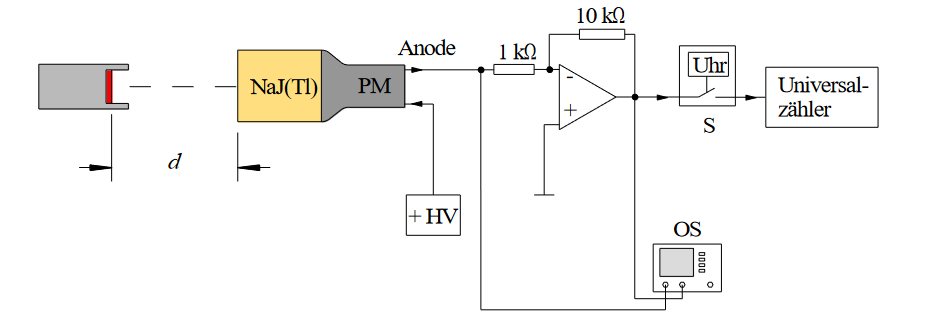
\includegraphics[width=0.7\textwidth]{2023-04-24 - V3 - Radioaktivität/images/versuch1/aufbau1.png}
    \caption{Schematischer Aufbau des Versuches, entnommen aus \cite{script}}
    \label{aufbau1}
\end{figure}
Der Photomultiplier des Detektors wird mit 1100 V von dem Hochspannungsgerät HV versorgt und die ausgehenden Signale werden mit einem Operationsverstärker verstärkt (die verwendeten Widerstände haben 10,06 $k\Omega$ und 1,012 $k\Omega$) und es werden beide Signale am Oszilloskop dargestellt. Der Aufbau ist mit einer Uhr und einem Universalzähler verbunden. Jedes Strahlungsereignis in dem an der Uhr eingestelltem Zeitraum wird an dem Zähler detektiert. Es wird die Hintergrundstrahlung gemessen, welche später aus der anderen Messung rausgerechnet wird. Dazu wird eine Messung für eine Zeit $\Delta t_0=120$ $s$ durchgeführt. Aus der mit dem Universalzähler gemessenen Impulszahl $M_0=8705$. Dadurch ergibt sich für $m_0=\frac{M_0}{\Delta t_0}=72,54$ $1/s$.
\end{document}
    \newpage
    % !TeX root = ..\protokoll.tex
\documentclass[../protokoll.tex]{subfiles}
\graphicspath{{\subfix{../images/}}}
\begin{document}
\section{Abstandsgesetz}\label{sec:Abstandsgesetz}
Bei dem Versuch des Abstandgesetzes soll die Quelle Cs-137 in einem Abstand von $d=d_1 +a (2,3,4,5,6,7,8,9,10,15,20,25,30,35,40)$ vom Szintillationsdetektor gemessen werden. Die Ergebnisse der Messung sollen dann für n(d) doppelt-logarithmisch über d aufgetragen werden und ein nicht linearer Kurven fit aufgetragen werden, mit der Gleichung (19) aus dem Skript als Zielfunktion, wobei $n_1$ als einziger freier Parameter anzunehmen ist und $r_0$ als festen Parameter. 
\begin{equation}
    n(d)=n_1(1-\frac{d}{\sqrt{r_0^2 + d^2}})
\end{equation}
Die Bestimmung der benötigten netto Zählrate erfolgt über die Gleichung (15) aus dem skript welche wie folgt lautet 
\begin{equation}
    n=m-m_0=\frac{M}{\Delta t}-\frac{M_0}{\Delta t_0}
\end{equation}
welche eine netto Zählrate von 554,94 ergibt.
\begin{figure}[H]
    \centering
    \includegraphics[width=0.7\textwidth]{2023-04-24 - V3 - Radioaktivität/images/Nicht linearer fit .png }
    \caption{n(d) über d aufgetragen, mit der Anpassung eines nicht linearen Fits nach Gleichung 19}
    \label{Abb.1}
\end{figure}
\begin{table}[H]
\centering
\begin{tabular}{|l|l|l|}
\hline
Abstand d=d\_1+a /cm & Messzeit  t/s & Zählrate  M \\ \hline
2                    & 100           & 199270      \\ \hline
3                    & 100           & 143775      \\ \hline
4                    & 100           & 108679      \\ \hline
5                    & 100           & 85864       \\ \hline
6                    & 100           & 69109       \\ \hline
7                    & 100           & 56230       \\ \hline
8                    & 100           & 47833       \\ \hline
9                    & 100           & 40479       \\ \hline
10                   & 100           & 35486       \\ \hline
15                   & 100           & 20656       \\ \hline
20                   & 100           & 14492       \\ \hline
25                   & 100           & 11140       \\ \hline
30                   & 100           & 9621        \\ \hline
35                   & 100           & 8152        \\ \hline
40                   & 100           & 7359        \\ \hline
\end{tabular}
\end{table}
Wie zusehen ist, sind die Messwerte sehr nahe am Linearen fit angelegt, sind in der Abbildung \ref{Abb.1} und sich dies auch durch Einsetzen der Werte in die Gleichung bestätigt. Es lässt sich auch noch am Grafen erkennen, dass trotz der doppelt logarithmischen Auftragung die Funktion doch noch einen leichten nicht linear ähnlichen Verlauf in der Abbildung aufweist wie in den vorherigen Versuchen, wo durch das doppelt logarithmischen Auftragen die Funktionen immer recht linear dargestellt werden konnten.
\end{document}
    
    \newpage
    \part{Anhang und Quellenverzeichnis}
    \printbibliography[heading=bibnumbered,title=Referenzen und Literatur]
    
\end{document}